\chapter{Trie}


\section{Data Structure}
\subsection{Basic}

\begin{figure}[hbtp]
\centering
\subfloat{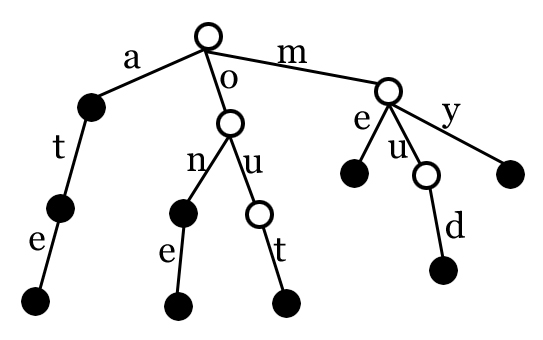
\includegraphics[scale=.30]{trie.jpg}}
\caption{Trie}
\label{fig:trie} 
\end{figure}

Notice:
\begin{enumerate}
\item Children are stored in HashMap rather than ArrayList. 
\item self.word to stores the word and indicates whethere a word ends at the current node. 
\end{enumerate}
Code: 
\begin{lstlisting}[language=python]
class TrieNode(object):
    def __init__(self, char):
        self.char = char
        self.word = None
        self.children = {}  # map from char to TrieNode


class Trie(object):
    def __init__(self):
        self.root = TrieNode(None)

    def add(self, word):
        word = word.lower()
        cur = self.root
        for c in word:
            if c not in cur.children:
                cur.children[c] = TrieNode(c)
            cur = cur.children[c]
        cur.word = word
\end{lstlisting}

\subsection{Advanced}
Notice:
\begin{enumerate}
\item Implicitly stores the current word. 
\item Implicitly stores the current char. 
\item When insert new word, do not override the existing TrieNode. A flag to indicate whether there is a word ending here.
\end{enumerate}
Code:
\begin{lstlisting}[language=python]
class TrieNode:
    def __init__(self):
        self.ended = False
        self.children = {}


class Trie:
    def __init__(self):
        self.root = TrieNode()

    def insert(self, word):
        cur = self.root
        for w in word:
            if w not in cur.children:   # not override
                cur.children[w] = TrieNode()
            cur = cur.children[w]

        cur.ended = True

    def search(self, word):
        cur = self.root
        for w in word:
            if w in cur.children:
                cur = cur.children[w]
            else:
                return False

        if not cur.ended:  # not ended here
            return False

        return True

    def startsWith(self, prefix):
        cur = self.root
        for w in prefix:
            if w in cur.children:
                cur = cur.children[w]
            else:
                return False

        return True
\end{lstlisting}
\subsection{Application}
\begin{enumerate}
\item Word search in matrix.
\item Word look up in dictionary.
\end{enumerate}


